\documentclass[]{report}

\usepackage[T1]{fontenc}
\usepackage[urw-garamond]{mathdesign}
\usepackage{garamondx}
\usepackage{amsmath, amsthm, amsfonts}
\usepackage[a4paper, total={4in, 8in}]{geometry}
\usepackage{tikz-cd} % used to draw commutative diagrams
\usepackage{graphicx}
\usepackage{hyperref}
\usepackage{mathtools}

% user defined commands go here
\newtheorem{theorem}{Theorem}[section]
\newtheorem{prop}[theorem]{Proposition}
\newtheorem{corollary}{Corollary}[theorem]
\newtheorem{lemma}[theorem]{Lemma}
\newtheorem{defn}[theorem]{Definition}
\newtheorem{examples}[theorem]{Example}
\newtheorem{exercise}[theorem]{Exercise}

\DeclareMathOperator\Spec{Spec}
\DeclareMathOperator\Max{Max}
\DeclareMathOperator\Ker{Ker}
\DeclareMathOperator\Coker{Coker}
\renewcommand{\qedsymbol}{$\blacksquare$}

\begin{document}

\title{%
    Introduction to Commutative Algebra: \\
    
    \large and affine algebraic varieties}
\author{Amal M}
\date{January 4, 2021}
\maketitle

\begin{abstract}

    The motivation for the study of algebraic geometry is how algebraic objects (rings of rational functions) are associated with varieties (zeros of polynomials). This subject florished during the second half of the twentieth century. Algebraic geometry allows us to study the geometry arising from algebraic objects. Core to the deeper understanding of this subject is an understanding of the subject of commutative algebra which studies commutative rings and their ideals and modules. The purpose of the present project is to gain an understanding of commutative algebra through solving exercises from Atiyah-MacDonald's book, Introduction to Commutative Algebra. The reading project comprised of the study of the theory of rings and modules, their tensor product and exact sequences of rings and modules. The project concluded with a proof of the Going-Up Theorem.

\end{abstract}

\tableofcontents
\newpage

\chapter{Introduction}

The purpose of the current project is to give an understanding 
to the reader of how commutative algebra is used to define the basic
objects of algebraic geometry. Algebraic Geometry is the study of
the geometric properties of the solution set of polynomial equations
in arbitary variables. For this purpose it is useful to confine the 
discussion to algebraically closed fields $k$ and the polynomial ring
$k[x_1,\cdots,x_n]$. We define \textit{affine n-space} over the algebraically closed field $k$ as $k^n$ and denote it by $\mathbb{A}^n_k$.

\begin{defn} The algebraic variety \cite{vakil145} in the affine space $\mathbb{A}^n_k$ of a set $S$ of polynomials $f\in k[x_1,\cdots, x_n]$, is a subset $V(S)\subseteq \mathbb{A}^n_k$ cut out by the set of mutual zeros of all the polynomials in the set $S$.  
    $$V(S) = \{x = (x_1,\cdots,x_n) \in \mathbb{A}^n_k : f(x) = 0 \text{ for all } f \in S\}.$$
\end{defn}

The affine variety is not the only example of a variety. The projective variety defined over projective spaces $\mathbb{P}^n_k$ is another example of an algebraic variety.

The solution set or \textit{locus} of solutions of polynomials of degree one are discrete points in $k$. But over $k^2$ the \textit{locus} are curves. For example, the solution of the elliptic curve given by the polynomial equation in $\mathbb{R}[x,y]$ in $\mathbb{R}^2$  
    $$y^2 = x^3 - 3x + 5$$
    is a curve (Fig 1.). The question then arises: \textit{what does the solution set of a set of polynomials in $k^3$ look like? What about $k^n$?} This is same asking the question: \textit{what does an affine algebraic variety in $\mathbb{A}^n_k$ look like?} We may go further by demanding: \textit{what is the topology of the affine algebraic variety?} (The answer is called the \textit{Zariski Topology}, which we shall get to in due time.)

    Once we have an affine algebraic variety we may define functions on them and we may define functions from one algebraic variety to another. Thus we start to do the usual mathematical \textit{shtick} on affine varieties.

    To answer the proposed questions we need to know the properties of an affine algebraic varieties. For example: \textit{what is so algebraic about an affine algebraic variety?} The answer is that we may consider every \textit{affine algebraic variety} to be some \textit{finitely generated nilpotent-free $k$-algebra $A$}. To know what each of these terms means we first need some commutative algebra. The purpose of this article is to explain these terms and give a brief introduction to Algebraic Geometry focusing only on affine algebraic varieties.

    The exposition is based on the knowledge gained after spending many hours working out the exercises contained in \cite{atiyah1}. I would advise anyone thinking about learning algebraic geometry to start there and work out those exercises themselves.  

    We divide the article into four sections. In the first section we introduce the \textit{prime spectrum} of a ring $A$, $X = \Spec(A)$ by which we denote the set of all prime ideals of $A$. We endow this space $X$ with a topology called \textit{the Zariski Topology}.

    In the next section, we introduce \textit{modules}, which are a sort of generalised vector spaces and \textit{algebras}, which are modules on rings, and we define the tensor product on a collection of such \textit{modules}. Then we discuss a particular sort of structure that can be given to a collection of modules called \textit{the direct limit} -- a term loaned from Category Theory. 

    In the third section we introduce the \textit{rings of fractions} of modules and the concept of \textit{localization} which we use in the formulation of a sort of structure called \textit{presheaf} and \textit{sheaf}. We also introduce the \textit{constructible topology} and the precise condition under which this topology is equivalent to the \textit{Zariski Topology} on $\Spec(A)$. 

    In the final section we introduce integral dependence, that is elements of rings that are integral over a subring and discuss the proof of the Going-Up Theorem, one of the two well known theorems of Cohen-Seidenberg. 

    % Start by giving an overview of the table of content

\begin{figure}
  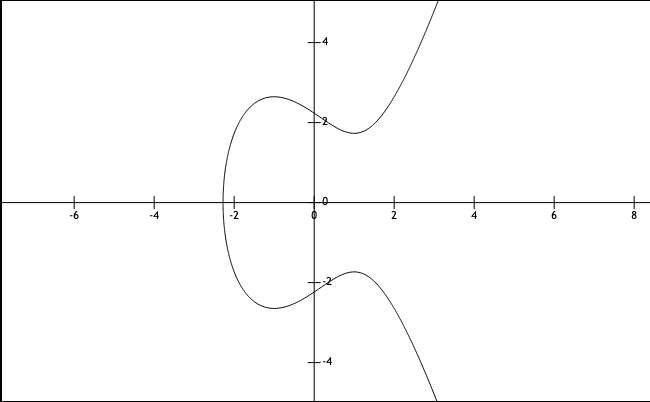
\includegraphics[width=\linewidth]{img/ell_curv1.png}
  \caption{Fig 1.}
  \label{fig:ell_curv1}
\end{figure}

\chapter {The Zariski Topology}

In commutative algebra what we generally call a \textit{ring} is a ring with unity, i.e, $1\in A$. So from now on, when we say ring we mean a set $A$ with two binary operations on it's elements $a + b \text{ and } a\dot b$, for all $a,b\in A$ such that A is an abelian group with respect to addition and multipication is associative and distributive over addition and $1\in A$ is the unique identity element.

A \textit{unit} in a ring $A$ is an element $x\in A$ such that there is another element $y\in A$ so that $xy = 1$. A ring in which every element is a \textit{unit} is called a \textit{field}. 

An element $x\in A$ is a \textit{nilpotent} element if $x^n = 0$ for some $n>0$. An element $x$ is an \textit{idempotent} element if $x^2 = x$. 

If we are given a group we know that if we quotient it by a normal subgroup we obtain another group and that the kernal of a group homomorphims is always a normal subgroup. Similarily rings have \textit{ideals}. Using \textit{ideals} can form a quotient ring and we have the fact that the kernal of every ring homomorphim is an ideal. 

\begin{defn}
    A subset $\mathfrak{a} \subseteq A$ is called an \textit{ideal} of $A$ if $\mathfrak{a}$ is an additive subgroup and it has the property, $y\in \mathfrak{a}$ and $x\in A$ implies $xy\in \mathfrak{a}$.
\end{defn}

Once we undersand what an ideal is we can define a \textit{prime ideal} of $A$ which is an ideal $\mathfrak{p}$ of $A$ with the property that $xy\in \mathfrak{p} \implies x \in \mathfrak{p} \text{ or } y\in \mathfrak{p}$. Similarily an ideal $\mathfrak{m}$ in A is \textit{maximal} if $\mathfrak{m} \neq (1)$ and if there is no ideal $\mathfrak{a}$ such that $\mathfrak{m\subset a\subset} (1)$. If we understand that given an ideal $\mathfrak{a}$ of a ring $A$ we can form the quotient ring $A/\mathfrak{a}$, we can look at the following proposition given without proof

\begin{prop}
    $$\mathfrak{p} \text{ is prime } \Leftrightarrow A/\mathfrak{p} \text{ is an integral domain }$$
    $$\mathfrak{m} \text{ is maximal } \Leftrightarrow A/\mathfrak{m} \text{ is a field }$$
\end{prop}

Therefore every \textit{maximal ideal} is a \textit{prime ideal} but the converse is not true in general. The reason prime ideals and maximal ideals are so important is because they have "nice" properties when we transport them across ring homomorphims. For example given a ring homomorphim $f:A\rightarrow B$ and a prime ideal $\mathfrak{q}\subset B$ the set $f^{-1}(\mathfrak{q})$ is a prime ideal  $\mathfrak{p}\subset A$. This result will be useful later on. Meanwhile we move onto the other memebers of \textit{ring theory}. 

A ring with just one \textit{maximal} ideal $\mathfrak{m}$ is called a \textit{local ring}. The quotient ring $k = A/\mathfrak{m}$ which is a field, is called the \textit{residue field} of $A$. 

\begin{defn}
    The radical of an ideal $\mathfrak{a}\subset A$ is another ideal 
    $$r(\mathfrak{a}) = \{x\in A: x^n\in \mathfrak{a} \text{ for some } n>0\}$$
\end{defn}

We can show that the \textit{radical} of an ideal is the intersection of all prime ideals that contain that ideal. If $x$ is an element of $\mathfrak{a}$ and if $x$ is any power of an element then that element belongs to the \textit{radical}. So the \textit{radical} is a way to associate elements related to $\mathfrak{a}$ by it's power. That is, if $f^n\in \mathfrak{a}$ then by definition of an ideal all the powers of $f$ higher than $n$ also belongs to $\mathfrak{a}$, the \textit{radical} ideal includes \textit{lower powers} of $f$ such as $f^{n-2}, f^{n-5}$ and so on. So we can have all powers of $f$ in $r(\mathfrak{a})$. 

We just need to define one more concept before we can move on to define the \textit{prime spectrum} of a ring. 

\begin{prop}
    The set $\mathfrak{N}$ of all nilpotent elements in a ring A is an ideal and $A/\mathfrak{N}$ has no nilpotent element $\neq 0$. \cite{atiyah1}
\end{prop}

The \textit{nilradical} of a ring $A$ has the property that it is equal to the intersection of all the prime ideals of $A$. It's worth asking the question: \textit{What is the intersection of all maximal ideals of $A$?}. The answer is precisely the \textit{Jacobson ideal} of $A$ denoted by $\mathfrak{R}$. It has the following property

\begin{prop}
    $x\in \mathfrak{R} \Leftrightarrow 1-xy$ is a unit in A for all $y\in A$. \cite{atiyah1}
\end{prop}

\section{Prime Spectrum}

The \textit{prime spectrum} of a ring is the set of all \textit{prime} ideals of the ring $A$ and we denote it by $X = \Spec(A)$. We consider this set to be a space in the following way. Each \textit{prime ideal} $\mathfrak{p}_x \in \Spec(A)$ is a point which we denot by $x$.

A topology on a space can be axiomatically defined using just the closed sets. We claim that for each subset $E$ of $A$
    $$V(E) = \{\mathfrak{p}\in \Spec(A): E\subseteq \mathfrak{p}\}$$
    satisfies the axioms for closed sets. To see this by Ex 15.ii $V(0) = X$ and $V(1) = \varnothing$. By 15.iii arbitary intersection of closed sets are seen to be closed. By 15.iv along with 15.i we can see that union of finitely many closed sets is closed. So the sets $V(E)$ do indeed form a topology on $\Spec(A)$. This topology is called \textit{the Zariski Topology}.

    This is not the only topology on $\Spec(A)$ we will discuss another such topology, the \textit{constructible topology}, later on. But for now we focus on the properties of the \textit{Zariski Topology}.

    The sets $X_f = X - V(f)$ are open sets in $X$ for each $f\in A$ since each $V(f)$ is closed. The family of such sets, $\{X_f\}_{f\in A}$ is the basis (Ex 17) of the \textit{Zariski Topology} and we call them the \textit{basic open sets} of $X$.

    $X$ is \textit{quasi-compact}. Which is exactly the same as \textit{compactness} in regular topology. For some reason Algebraic Geometers do not use the term \textit{compactness} to mean just the condition \textit{every open cover has a finite subcover}. But instead a space is \textit{compact} if it is also Hausdorff as well as \textit{quasi-compact}. This is because every $\Spec(A)$ has the usual property of having a finite subcover for an open covering. So just calling it \textit{compact} is a waste of a perfectly good word that can be used for something more significant. 

    We find that every open set $X_f$ is quasi-compact as well every finite union of sets $X_f$. Indeed we have that a subset of $X$ is quasi-compact if and only if it is a union of finitely many open sets $X_f$ (Ex 17.vii).

    A singleton set $\{x\}$ in the Zariski Topology is closed if and only if $\mathfrak{p}_x$ is maximal (Ex 18.i). $X$ is also $T_0$-space.

    Now would be a good time to see some examples of the \textit{prime spectrum} of some well known rings such as $\mathbb{Z, R, C}[x]$ and $\mathbb{Z}[x]$ (Ex 16).



\section{Maximal Spectrum}

The \textit{maximal spectrum} of a ring is the set of all \textit{maximal} ideals of the ring. It is denoted by $\Max(A)$. The \textit{maximal spectrum} is a subset of the \textit{prime spectrum} $\Spec(A)$. We can quickly give a concrete example for a \textit{maximal spectrum}.

Let $X$ be a compact Hausdorff space and let $C(X)$ be the ring of all real valued continuous functions on $X$. Define
$$\mathfrak{m}_x = \{f\in C(X): f(x) = 0\}$$
Then $\mathfrak{m}_x$ is an ideal and furthermore it is a maximal ideal since if we define a function $\phi_x: C(X) \rightarrow \mathbb{R}$ as the mapping $f\mapsto f(x)$ then the kernel of the map is $\mathfrak{m}_x$. 

Let $\hat{X} = \Max(A)$ we can define a mapping $\mu: X\rightarrow \hat{X}$ by $x\mapsto \mathfrak{m}_x $. By Ex 26.i $\mu$ is surjective and by Ex 26.ii it is injective. Let $f\in C(X)$ and define
$$U_f = \{x\in X:f(x) = 0\}$$
$$\hat{U}_f = \{\mathfrak{m}\in \hat{X}:f\not\in \mathfrak{m}\}$$
We can show that $\mu(U_f) = \hat{U}_f$ (Ex 27.iii). So $\mu$ sends the basis of $X$ the basis of $\hat{X}$ and so $\mu$ is a homeomorphism.

We have just show that given only the functions on a compact Hausdorff space $X$ we can reconstruct the underlying space.

\section{Affine Algebraic Varieties}

Given a set $S$ of polynomial in $k[x_1,\cdots,x_n]$ we have defined the \textit{affine algebraic variety} on $S$ as the subset $V(S)$ of the affine space $\mathbb{A}^n_k$.
$$V(S) = \{x = (x_1,\cdots,x_n) \in \mathbb{A}^n_k : f(x) = 0 \text{ for all } f \in S\}.$$
Now we consider the opposite behavior? 

Given a subset $X$ of the affine space we define the \textit{ideal of the variety} $X$ to be the set of polynomials $g\in k[x_1,\cdots,x_n]$ that vanish on $X$. It is denoted by $I(X)$.
$$I(X) = \{g\in k[x_1,\cdots,x_n]: g(x) = 0, \forall x\in X\}$$
This set is an ideal since if two polynomials $f,g\in I(X)$ then $f+g\in I(X)$ as the sum of the polynomials vanish if they each individually vanish and for any polynomial $f \in k[x_1,\cdots, x_n]$ and $g\in I(X)$, $fg = 0$ so $fg\in I(X)$ as well.

    The quotient ring
    $$P(X) = k[x_1,\cdots,x_n]/I(X)$$
    is called the ring of polynomial functions on $X$. If two polynomials $f$ and $g$ belong to the same coset, then $f-g \in I(X)$ that means over $X$, $(f-g)(x) = 0$, i.e., the two polynomials agree in value over $X$. So the polynomial ring contains only distinct polynomials over $X$.

    Let $\xi_i$ be the image in $P(X)$ of $x_i$. Then the $x_i (1\leq i\leq n)$ are called the \textit{coordinate functions} on $X$. $P(X)$ is generated as a $k$-algebra by the \textit{coordinate functions} and it is called the \textit{coordinate ring} or \textit{affine algebra} on $X$.

    For each $x\in X$ the ideal $\mathfrak{m}_x$ consiting of $f\in P(X)$ such that $f(x) = 0$ is a maximal ideal. Let $\hat{X} = \Max(P(X))$. We can use Hilbert's Nullstellensatz to show that the mapping $\mu: X \rightarrow \hat{X}$ given by $x\mapsto \mathfrak{m}_x$ is a bijection.

\subsection{Polynomial Functions}

Let $f_1,\cdots, f_m$ be $m$ polynomials in $k[x_1,\cdots,x_n]$. We can define a mapping $\phi: k^n\rightarrow k^m$ by $\phi(x) = (f_1(x),\cdots,f_m(x))$. Such a mapping is called a \textit{polynomial mapping}.

    Let $X,Y$ be affine algebraic varieties in $k^n$ and $k^m$ respectively. A mapping $\phi: Y\rightarrow X$ is a \textit{regular} mapping if $\phi$ is a restriction of a polynomial mapping from $k^n$ to $k^m$.

    $\phi$ induces a $k$-algebra homomorphim $P(Y) \rightarrow P(X)$ given by sending polynomial functions on $Y$ to their composition with $\phi$. Therefore there is a one-to-one correspondence between the regular mappings $X\rightarrow Y$ and the $k$-algebra homomorphim $P(Y) \rightarrow P(X)$.


\chapter{Tensor Product and Direct Limits}

Let $A$ be a ring. An $A$-\textit{module} is an abelian group $M$ along with a mapping $\mu: A\times M\rightarrow M$, $\mu(a,x)$ denoted by $ax, a\in A, x\in M$ which satisfies the following
\begin{enumerate}
    \item $a(x+y) = ax + ay$
    \item $(a+b)x = ax + bx$
    \item $(ab)x = a(bx)$
    \item $1x = x$, 
 ($\forall a,b \in A, \forall x,y \in M$.)
\end{enumerate}

A \text{module homomorphism} between two modules $M$ and $N$ is an $A$-linear mapping between two abelian groups $f:M\rightarrow N$, such that the following two properties are satisfied
\begin{enumerate}
    \item $f(x+y) = f(x) + f(y)$
    \item $f(a.x) = a.f(x)$
\end{enumerate}

A \textit{submodule} $M'$ of $M$ is a subgroup that is closed under multiplication by elements of $A$. The quotient $M/M'$ is also an A-module as it is the action of $A$ on the quotient is $a(x + M') = ax + M'$.

Given two modules $M$ and $N$, their direct product is given as the module $M\oplus N$ which is the set of all elements $(x,y), x\in M, y\in N$ with two operations defined on it
$$(x_1,y_1) + (x_2,y_2) = (x_1+x_2, y_1+y_2)$$
$$a(x,y) = (ax, ay)$$

Given an arbitary family of $A$-modules, $(M_i)_{i\in I}$ the direct sum of the family is the sum $\bigoplus_{i\in I} M_i$ is the set of all families $(x_i)_{i\in I}$, $x_i\in M_i$ such that all but finitely many $x_i$ are nonzero. It is a module by the same operation as above. 

A sequence of $A$-modules and $A$-homomorphisms,
$$\cdots \rightarrow M_{i-1} \xrightarrow{f_i} M_i \xrightarrow{f_{i+1}} M_{i+1} \rightarrow \cdots$$ 
is said to be \textit{exact} at $M_i$ if, $\Ker(f_{i+1}) = \text{Im}{f_i}$. The sequence is exact if it is exact at each $M_i$. 

\begin{enumerate}
    \item $0 \rightarrow M' \xrightarrow{f} M$ is exact $\Leftrightarrow$ $f$ is injective.
    \item $M \xrightarrow{g} M'' \rightarrow 0$ is exact $\Leftrightarrow$ $g$ is surjective. 
    \item $0 \rightarrow M' \xrightarrow{f} M \xrightarrow{g} M'' \rightarrow 0$ is exact $\Leftrightarrow$ $f$ is injective and $g$ is surjective. But also $\Coker(f) = M/f(M')$ is isomorphic to $M''$. This type of exact sequence is also called a short exact sequence. 
\end{enumerate}

A sequence of type (3) is called a \textit{short exact sequence}.

\section{Tensor Product}

The \textit{tensor product} of two $A$-modules $M$ and $N$ is the $A$-module $M\otimes N$ of all linear combination of the pair $x \otimes y$ with coefficients in $A$ along with the following properties,
\begin{enumerate}
    \item $(x + x') \otimes y = x \otimes y + x' \otimes y$
    \item $x \otimes (y + y') = x \otimes y + x \otimes y'$
    \item $a.x \otimes y = x \otimes a.y = a(x \otimes y)$
\end{enumerate}

We see that $0 \otimes x = x\otimes 0 = 0$ as $0.(a\otimes x) = 0$. If $x_i$ generates M and $y_i$ generates N then $x_i \otimes y_i$ generates $M\otimes N$. 

Let $x\in M$ and $y\in N$ if $M' \subseteq M$ and $N'\subseteq N$ are submodules then $x\otimes y \in M\otimes N$ is not the same as $x\otimes y \in M'\otimes N'$ 

To be specific the tensor product of A-modules is denoted by $M \otimes_A N$ but if the context is clear we can write $M\otimes N$.

\begin{prop} \cite{atiyah1}
    Let M,N,P be A-modules. Then there exists unique isomorphisms called the cannonical isomorphisms 
    \begin{enumerate}
        \item $M\otimes N \rightarrow N\otimes N$, (given by $x\otimes y \mapsto y\otimes x$)
        \item $(M\otimes N) \otimes P \rightarrow M\otimes (N\otimes P) \rightarrow M\otimes N\otimes P$, (given by $(x\otimes y) \otimes z \mapsto x \otimes (y\otimes z) \mapsto x\otimes y \otimes z$)
        \item $(M\oplus N) \otimes P \rightarrow (M\otimes P) \oplus (N\otimes P)$, given by $(x,y)\otimes z \mapsto (x\otimes z, y\otimes z)$
        \item $A\otimes M \rightarrow M$, given by $a\otimes x \mapsto ax$. 
    \end{enumerate}
\end{prop}
    
\section{Flatness}

A $A$-module $N$ is called a \textit{flat} module if for every exact sequence
$$\cdots \rightarrow M_{i-1} \xrightarrow{f_i} M_i \xrightarrow{f_{i+1}} M_{i+1} \rightarrow \cdots$$ 
when \textit{tensored} (multiplied) by $N$ gives another sequence
$$\cdots \rightarrow M_{i-1}\otimes N \xrightarrow{f_i} M_i\otimes N \xrightarrow{f_{i+1}} M_{i+1}\otimes N \rightarrow \cdots$$ 
which is \textit{exact}.

\section{Tensor Product of Algebras}

We now define multiplicaton on the tensor product in the following way so that it turns into a commutative ring with identity element $1\otimes 1$:

Let $B,C$ be two $A$-algebras with associated homomorphims $f:A\rightarrow B$ and $g:A\rightarrow C$. As algebras are themselves modules we take their tensor product $D = B\otimes_A C$. 

Define the multiplicaton $D\otimes D \rightarrow D$ by the A-bilinear mapping $\mu: D\times D \rightarrow D$ so that,
$$\mu(b\otimes c, b'\otimes c') = bb' \otimes cc'. $$


That is, $(b\otimes c)(b'\otimes c') = bb'\otimes cc'$ and more generally, $(\sum_i(b_i\otimes c_i))(\sum_j(b'_j\otimes c'_j)) = \sum_{i,j}(b_i b'_j \otimes c_i c'_j)$
\begin{enumerate}
    \item The mapping $a\mapsto f(a)\otimes g(a)$ is a ring homomorphism $A\rightarrow D$. 
    \item There is a commutative diagram of ring homomorphisms, 
\end{enumerate}

\begin{equation*}
    \begin{tikzcd}
                                  & B \arrow[rd, "u"] &   \\
        A \arrow[ru, "f"] \arrow[rd, "g"] &                   & D \\
                                  & C \arrow[ru, "v"] &  
    \end{tikzcd}
\end{equation*}


\section{Direct Limit}

The concept of a \textit{direct limit} comes from the Category Theory notion of \textit{colimits}. We put together a collection of modules to make another module which we shall use later.

Let $(M_i)_{i\in I}$ be a family of $A$-modules where the set $I$ has the property that that it is a partially ordered set as well as a \textit{directed set}, by which we mean that for each pair $i,j$ in $I$ there exists $k\in I$ such that $i\leq k$ and $j\leq k$. We also have for each pair $i,j$ in $I$ and $i\leq j$ the $A$-homomorphim $\mu_{ij}: M_i \rightarrow M_j$ which satisfies the following two properties
\begin{enumerate}
    \item $\mu_{ii}$ is the identity mapping $\forall i\in I$.
    \item $\mu_{ik} = \mu_{jk}\circ \mu_{ij}$ whenever $i\leq j\leq k$.
\end{enumerate}

$(M_i,\mu_{ij})$ is called the \textit{direct system} over the directed set $I$.

Given a \textit{direct system} what we shall do is take the direct sum over the modules $M_i$, that is $\bigoplus_{i\in I} M_i = C$. Then we define the submodule $D$ of $M$ to be the module which is generated by only such elements of the form
$$x_i - \mu_{ij}(x_i), \textit{ whenever } i\leq j.$$

Note that once we take the direct sum $C$ we can take every element $x_i\in M_i$ and talk about it being an element of $C$ in a natural way. Just think of $C$ as the set of all sum $x_1  + x_2 + \cdots$. Then $x_i + \mu_{ij}(x_i)$ is an element of $C$ and the submodule generated by all such elements is denoted as $D$. Now we take the quotient $C/D$ and we call it the \textit{direct limit} $M$.

There's nothing very sophisticated about the definition of the \textit{direct limit} even though it may seem complicated. If you understand direct sums very well the definition is straightforward. But what's difficult to see is why we need to have a \textit{direct limit} at all. The motivation for having the \textit{direct limit} is so that we can 


\chapter{Sheaf and Presheaf}
\section{Support}
\section{Presheaf}
\section{Sheaf}
\section{Constructible Topology}
\section{Absolute Flatness}

\chapter{The Going-Up Theorem}

\begin{thebibliography}{9}

\bibitem{vakil145}
    Ravi Vakil,
    \textit{Math 145: Algebraic Geometry}

\bibitem{atiyah1}
    Atiyah-Macdonald, 
    \textit{Introduction to Commutative Algebra}

\bibitem{treasuremap}
    Mumford's Treasure Map,
    \href{https://web.archive.org/web/20201130150255/http://www.neverendingbooks.org/mumfords-treasure-map}{\textit{Mumford's Treasure Map}}
\end{thebibliography}

\end{document}
